\ifx\wholebook\relax \else
\documentclass[b5paper]{ctexart}
\usepackage[nomarginpar
  %, margin=.5in
]{geometry}

\addtolength{\oddsidemargin}{-0.05in}
\addtolength{\evensidemargin}{-0.05in}
\addtolength{\textwidth}{0.1in}
\usepackage[cn]{../../../prelude}

\setcounter{page}{1}

\begin{document}

\title{队列}

\author{刘新宇
\thanks{{\bfseries 刘新宇 } \newline
  Email: liuxinyu95@gmail.com \newline}
  }

\maketitle
\fi

\markboth{队列}{基本算法}

\ifx\wholebook\relax
\chapter{队列}
\numberwithin{Exercise}{chapter}
\fi

\section{简介}
\label{introduction}

队列提供了先进先出(FIFO)的机制。可以用多种方法实现队列,例如单向、双向链表,循环缓冲区等,冈崎给出了16种不同的实现方法\cite{okasaki-book}。队列需要满足下面的两条基本要求:

\begin{enumerate}
\item 可以在常数时间内向末尾添加元素;
\item 可以在常数时间内从头部获取或删除元素。
\end{enumerate}

可以用双向链表直观地实现队列。我们略去这个简单的实现,而关注如何用其它基本数据结构,如列表、数组实现队列。

\section{列表实现}
\index{队列!单向链表实现}

我们可以用常数时间在列表头部插入、删除元素。但为了先进先出,我们只能在头部执行一种操作,而在尾部执行另一种操作。我们需要$O(n)$时间遍历整个列表以到达尾部,其中$n$是列表长度。这样就无法达到性能要求。为了解决这个问题,可以一个变量记录尾部位置。并用一个额外的节点$S$简化空队列的处理,如\cref{fig:empty-list}所示。

\lstset{frame = single}
\begin{lstlisting}[language = Bourbaki]
data Node<K> {
  Key key
  Node next
}

data Queue {
  Node head, tail
}
\end{lstlisting}

\begin{figure}[htbp]
  \centering
  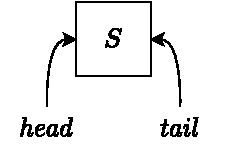
\includegraphics[scale=0.8]{img/empty-list}
  \caption{空队列,头、尾都指向$S$}
  \label{fig:empty-list}
\end{figure}

队列中最基本的两个操作是入队(Enqueue,或push、snoc、append、push back)和出队(Dequeue,或pop、pop front)。使用列表时,我们选择在头部加入元素、从尾部删除元素以简化实现。

\begin{algorithmic}[1]
\Function{Enqueue}{$Q, x$}
  \State $p \gets $ \Call{Node}{$x$}
  \State \Call{Next}{$p$} $\gets$ NIL
  \State \textproc{Next}(\Call{Tail}{$Q$}) $\gets p$
  \State \Call{Tail}{$Q$} $\gets p$
\EndFunction
\end{algorithmic}

队列至少有一个节点(空队列中有$S$节点),因此无需检查尾部是否为NIL。

\begin{algorithmic}[1]
\Function{Dequeue}{$Q$}
  \State $x \gets $ \Call{Head}{$Q$}
  \State \textproc{Next}(\Call{Head}{$Q$}) $\gets$ \Call{Next}{$x$}
  \If{$x = $ \Call{Tail}{$Q$}} \Comment{$Q$变为空}
    \State \Call{Tail}{$Q$} $\gets$ \Call{Head}{$Q$}
  \EndIf
  \State \Return \Call{Key}{$x$}
\EndFunction
\end{algorithmic}

$S$节点在所有其它节点的前面,\textproc{Head}实际返回$S$的下一个节点,如\cref{fig:list-queue}所示。我们可以把这一实现扩展到并发环境。在头部和尾部各使用一把并发锁。$S$节点可以在队列空时避免死锁\cite{PODC96}、\cite{SutterDDJ}。

\begin{figure}[htbp]
  \centering
  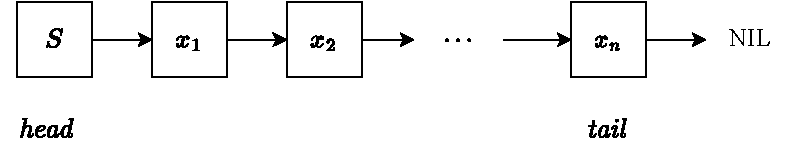
\includegraphics[scale=0.8]{img/slistq}
  \caption{带有$S$节点的列表}
  \label{fig:list-queue}
\end{figure}

\section{循环缓冲区}
\index{队列!循环缓冲区}

和列表相反,我们可以在常数时间将元素添加到数组末尾,但需要线性时间$O(n)$从头部删除。这是因为要将全部剩余元素依次向前移动。为了达到队列的性能要求,我们可以把数组的头尾连接起来,做成一个环,叫做循环缓冲区,如图如\cref{fig:circular-buffer}、\cref{fig:circular-buffer-queue}所示。这样用数组的头部坐标head,队列长度count,和数组大小size,就可以完全表述队列。count等于0时队列为空,等于size时队列已满。我们还可以利用模运算简化入队、出队的实现。

\begin{figure}[htbp]
 \centering
 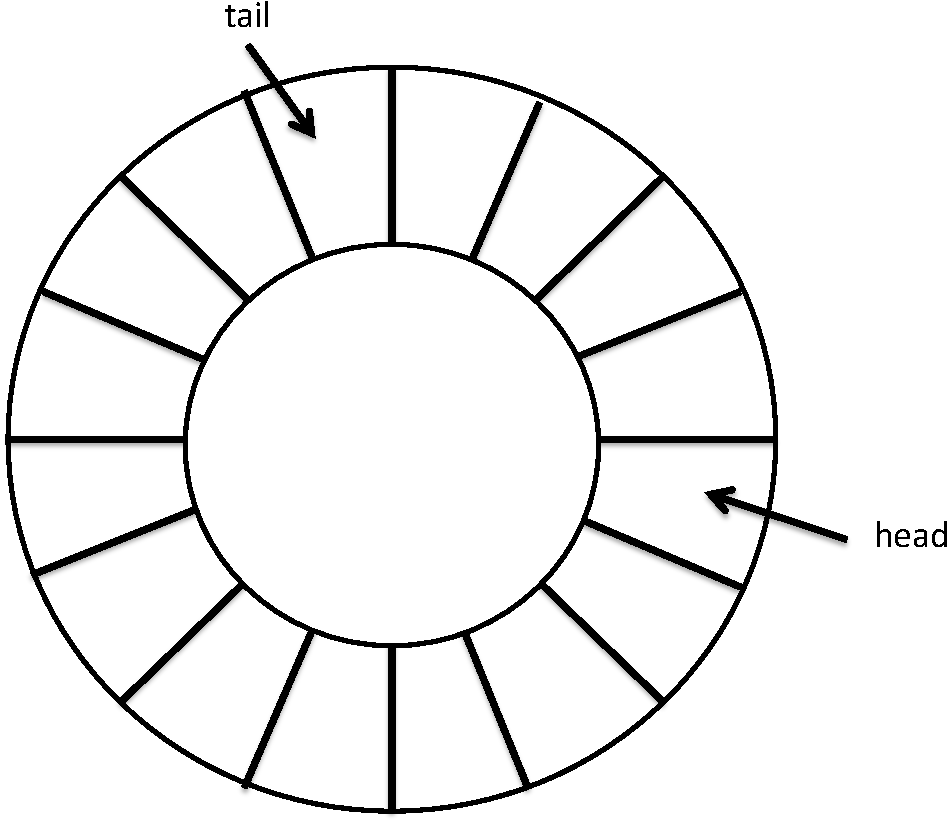
\includegraphics[scale=0.3]{img/ring-buffer}
 \caption{循环缓冲区}
 \label{fig:circular-buffer}
\end{figure}

\begin{figure}[htbp]
 \centering
 \subcaptionbox{连续加入多个元素。}{
 \begin{tikzpicture}[scale=0.8]
    \draw (0, 0) rectangle (1, 1) node (a0) [pos=.5] {a[0]}
          (1, 0) rectangle (2, 1) node [pos=.5] {a[1]}
          (2, 0) rectangle (3, 1) node [pos=.5] {...}
          (3, 0) rectangle (4, 1) node [pos=.5] (ai) {a[i]}
          (4, 0) rectangle (5, 1) node [pos=.5] {...}
          (5, 0) rectangle (6, 1) node (an) [pos=.5] {};
    \draw (0, 2) node (hd) {head}
          (3.5, 2) node (tl) {tail}
          (6, 2) node (bd) {边界};
    \draw[thick, ->] (hd) edge (a0)
                 (tl) edge (ai)
                 (bd) edge (an);
  \end{tikzpicture}}
 \subcaptionbox{从头部删除若干元素后,出现了空档。}{
  \begin{tikzpicture}[scale=0.8]
    \draw (0, 0) rectangle (1, 1)
          (1, 0) rectangle (2, 1) node [pos=.5] {...}
          (2, 0) rectangle (3, 1) node (aj) [pos=.5] {a[j]}
          (3, 0) rectangle (4, 1) node [pos=.5] {...}
          (4, 0) rectangle (5, 1) node (ai) [pos=.5] {a[i]}
          (5, 0) rectangle (6, 1) node [pos=.5] {...}
          (6, 0) rectangle (7, 1) node (an) [pos=.5] {};
    \draw (2, 2) node (hd) {head}
          (4.5, 2) node (tl) {tail}
          (7, 2) node (bd) {边界};
    \draw[thick, ->] (hd) edge (aj)
                 (tl) edge (ai)
                 (bd) edge (an);
  \end{tikzpicture}} \\
 \subcaptionbox{继续加入多个元素直到数组的边界。}{
   \begin{tikzpicture}[scale=0.8]
    \draw (0, 0) rectangle (1, 1)
          (1, 0) rectangle (2, 1) node [pos=.5] {...}
          (2, 0) rectangle (3, 1) node (aj) [pos=.5] {a[j]}
          (3, 0) rectangle (4, 1) node [pos=.5] {...}
          (4, 0) rectangle (5, 1) node (ai) [pos=.5] {a[i]};
    \draw (2, 2) node (hd) {head}
          (4.5, 2) node (tl) {tail}
          (6, 2) node (bd) {边界};
    \draw[thick, ->] (hd) edge (aj)
                 (tl) edge (ai)
                 (bd) edge [bend left] (ai);
  \end{tikzpicture}}
 \subcaptionbox{下一个元素加入到数组头部的第一个单元。}{
    \begin{tikzpicture}[scale=0.8]
    \draw (0, 0) rectangle (1, 1) node (a0) [pos=.5] {a[0]}
          (1, 0) rectangle (2, 1) node [pos=.5] {...}
          (2, 0) rectangle (3, 1) node (aj) [pos=.5] {a[j]}
          (3, 0) rectangle (4, 1) node [pos=.5] {...}
          (4, 0) rectangle (5, 1) node (an) [pos=.5] {};
    \draw (2.5, 2) node (hd) {head}
          (0, 2) node (tl) {tail}
          (6, 2) node (bd) {边界};
    \draw[thick, ->] (hd) edge (aj)
                 (tl) edge (a0)
                 (bd) edge (an);
  \end{tikzpicture}} \\
 \subcaptionbox{全部单元都保存了元素,队列已满。}{
   \begin{tikzpicture}[scale=0.8]
    \draw (0, 0) rectangle (1, 1) node [pos=.5] {a[0]}
          (1, 0) rectangle (2, 1) node [pos=.5] {a[1]}
          (2, 0) rectangle (3, 1) node [pos=.5] {...}
          (3, 0) rectangle (4, 1) node (a1j) [pos=.5] {a[j-1]}
          (4, 0) rectangle (5, 1) node (aj) [pos=.5] {a[j]}
          (5, 0) rectangle (6, 1) node [pos=.5] {...}
          (6, 0) rectangle (7, 1) node (an) [pos=.5] {};
    \draw (4.5, 2) node (hd) {head}
          (3, 2) node (tl) {tail}
          (7, 2) node (bd) {边界};
    \draw[thick, ->] (hd) edge (aj)
                 (tl) edge (a1j)
                 (bd) edge (an);
  \end{tikzpicture}}
 \caption{使用循环缓冲区实现队列} \label{fig:circular-buffer-queue}
\end{figure}

\begin{algorithmic}[1]
\Function{Enqueue}{$Q, x$}
  \If{not \Call{Full}{$Q$}}
    \State \Call{Count}{$Q$} $\gets$ \Call{Count}{$Q$} + 1
    \State tail $\gets $ (\Call{Head}{$Q$} + \Call{Count}{$Q$}) $\bmod$ \Call{Size}{$Q$}
    \State \Call{Buf}{$Q$}[tail] $\gets x$
  \EndIf
\EndFunction
\end{algorithmic}

\begin{algorithmic}[1]
\Function{Dequeue}{$Q$}
  \State $x \gets$ NIL
  \If{not \Call{Empty}{$Q$}}
    \State $h \gets$ \Call{Head}{$Q$}
    \State $x \gets$ \Call{Buf}{$Q$}[$h$]
    \State \Call{Head}{$Q$} $\gets $ (h + 1) $\bmod$ \Call{Size}{$Q$}
    \State \Call{Count}{$Q$} $\gets$ \Call{Count}{$Q$} - 1
  \EndIf
  \State \Return $x$
\EndFunction
\end{algorithmic}

\begin{Exercise}\label{ex:buffered-queue}
循环缓冲区在初始化时规定了最大的容量,如果使用头、尾两个指针,而不用Count,如何检测队列是否为空?是否已满?
\end{Exercise}

\begin{Answer}[ref = {ex:buffered-queue}]
循环缓冲区在初始化时规定了最大的容量,如果使用头、尾两个指针,而不用Count,如何检测队列是否为空?是否已满?

尽管可以分别考虑头部在尾部前面,和头部在尾部后面的情况,如\cref{fig:circular-buffer-queue},我们思考更简单一致的方法。考虑向左右两侧无限伸展的区域,记头部索引为$h$、尾部为$t$、缓冲区容量为$s$。左闭右开区间$[h, t)$被内容占据。空、满判断条件如下:

\[
\begin{cases}
empty(h, t): & h = t  \\
full(h, t): & t - h = s \\
\end{cases}
\]

循环缓冲区相当于在此基础上引入了模运算(时钟运算),记$[n]_s = n \bmod s$。对上述判满条件取模就会发现:$[t]_s - [h]_s = [s]_s = 0$,即$[t]_s = [h]_s$。这恰恰是判空条件取模的结果。因此,仅仅用头尾取模后的结果比较是无法判断队列空、满的。我们要么引入一个标记(标记$h$、$t$的先后顺序),要么在空、满判定时不取模,而仅仅在索引元素时取模。如果考虑实际实现时的整数字长限制,可以用一个和$s$互素的大数$p$($p > s$)取模进行判定,即:

\[
\begin{cases}
empty(h, t): & [h]_p = [t]_p  \\
full(h, t): & [t - h]_p = s \\
\end{cases}
\]

例子程序:

\begin{Bourbaki}
Int P_LIMIT = 104743 // the 10000th prime
Bool empty(Queue<K> q) = (q.h == q.t)
Bool full(Queue<K> q) = (q.s == (q.t - q.h) mod P_LIMIT)

void enqueue(Queue<K> q, K x) {
    if not full(q) {
        q.t = (q.t + 1) mod P_LIMIT
        q.buf[q.t mod q.s] = x
    }
}

Optional<K> dequeue(Queue<K> q) {
    Optional<K> x = Optional.Nothing
    if not empty(q) {
        x = Optional.of(q.buf[q.h mod q.s])
        q.h = (q.h + 1) mod P_LIMIT
    }
    return x
}
\end{Bourbaki}
\end{Answer}

\section{双列表队列}
\index{队列!双列表队列}

列表的头部操作为常数时间,但尾部需要线性时间。我么可以把两个列表“尾对尾”连起来实现队列。形状类似一个马蹄形磁铁,如\cref{fig:horseshoe-magnet}所示。两个列表分别叫做前(front)和后(rear)。队列记为$(f, r)$,空队列等于$([\ ], [\ ])$。我们把新元素加入$r$的头部,出队时,将元素从$f$的头部取走,性能都是常数时间。

\begin{figure}[htbp]
  \centering
  %\subcaptionbox{马蹄形磁铁}{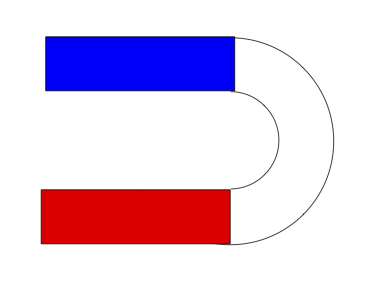
\includegraphics[scale=0.4]{img/horseshoe-magnet}} \\
  %\subcaptionbox{“尾对尾”接在一起的列表}{
    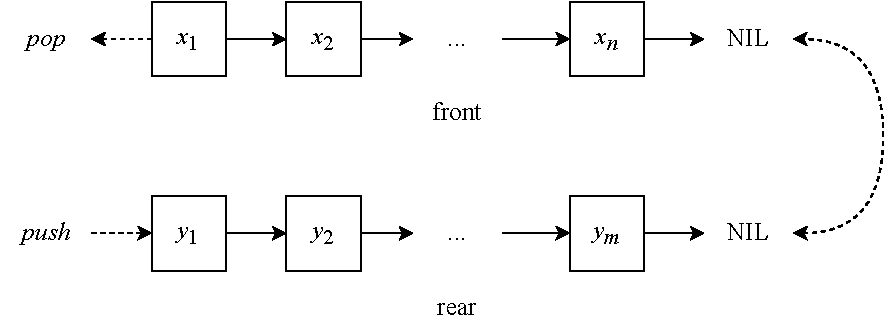
\includegraphics[scale=0.6]{img/paired-listq}
  %}
  \caption{双列表队列}
  \label{fig:horseshoe-magnet}
\end{figure}

\be
\begin{cases}
push\ x\ (f, r) & = (f, x \cons r) \\
pop\ (x \cons f, r)   & = (f, r) \\
\end{cases}
\ee

经过一系列出队操作后,$f$可能为空,而$r$中还有元素。为了能继续出队,我们将$r$反转后替换掉$f$,即:$([\ ], r) \mapsto (reverse\ r, [\ ])$。为此每次出入队后,需要执行一次平衡检查和调整:

\be
\begin{array}{rcl}
\textit{balance}\ [\ ]\ r & = & (\textit{reverse}\ r, [\ ]) \\
\textit{balance}\ f\ r & = & (f, r) \\
\end{array}
\ee

一旦发生$r$的反转,则这次操作的性能下降为线性时间。尽管如此,整体的分摊复杂度是常数时间的。我们重新定义入队和出队为:

\be
\begin{cases}
push\ x\ (f, r) & = \textit{balance}\ f\ (x \cons r) \\
pop\ (x \cons f, r)   & = \textit{balance}\ f\ r \\
\end{cases}
\ee

\index{队列!双数组队列}
我们可以用数组给出一个双列表的对称实现。利用\cref{tab:array-list-comp}的对称性,我们将两个数组“头对头”连接起来形成队列,如\cref{fig:horseshoe-array}所示。当$R$数组为空时,我们将$F$数组反转替换掉$R$数组。

\begin{table}[htbp]
\centering
\begin{tabular}{l | c | r}
  \hline
  操作 & 数组 & 链表 \\
  \hline
  在头部加入 & $O(n)$ & $O(1)$ \\
  在尾部加入 & $O(1)$ & $O(n)$ \\
  在头部删除 & $O(n)$ & $O(1)$ \\
  在尾部删除 & $O(1)$ & $O(n)$ \\
  \hline
\end{tabular}
\caption{数组和链表各项操作的对比} \label{tab:array-list-comp}
\end{table}

\begin{figure}[htbp]
  \centering
  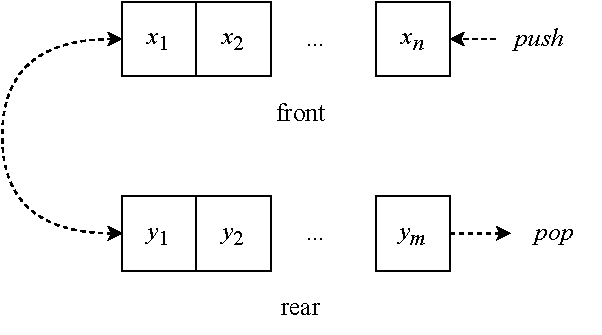
\includegraphics[scale=0.6]{img/paired-arrayq}
  \caption{双数组队列}
  \label{fig:horseshoe-array}
\end{figure}

\begin{Exercise}\label{ex:paired-list-queue}
\Question{为什么要在push时也要进行平衡检查和调整?}
\Question{试分析双列表队列的分摊复杂度。}
\Question{实现双数组队列。}
\end{Exercise}

\begin{Answer}[ref = {ex:paired-list-queue}]
\Question{为什么要在push时也要进行平衡检查和调整?

考虑这样的情况:先$push\ a\ ([\ ], [\ ])$,然后再$pop$。
}
\Question{试分析双列表队列的分摊复杂度。

我们使用记账法分析。尾部列表$r$中的每个元素记1分。向尾部列表push,执行一次加入操作,并增加1分。分摊消耗为$O(2)$。每次pop,如果未造成列表反转,则执行一次取出操作,但没有增减分数。分摊消耗为$O(1)$。如果造成列表反转,则执行$m$次反转和1次取出,其中$m$是尾部列表$r$的长度,并且使用了$r$列表中的$m$分。所以分摊消耗为$O(m + 1 - m) = O(1)$。
}
\Question{实现双数组队列。

\begin{algorithmic}[1]
\Function{Push}{$Q, x$}
  \State \textproc{Append}(\Call{Front}{$Q$}, $x$)
\EndFunction
\Statex
\Function{Pop}{$Q$}
  \If{\Call{Rear}{$Q$} $= [\ ]$}
    \State \Call{Rear}{$Q$} $\gets$ \textproc{Reverse}(\Call{Front}{$Q$})
    \State \Call{Front}{$Q$} $\gets [\ ]$
  \EndIf
  \State $n \gets$ \textproc{Length}(\Call{Rear}{$Q$})
  \State $x \gets$ \Call{Rear}{$Q$}[n]
  \State \textproc{Length}(\Call{Rear}{$Q$}) $\gets n - 1$
  \State \Return $x$
\EndFunction
\end{algorithmic}

}
\end{Answer}

\section{平衡队列}
\index{队列!平衡队列}

虽然双列表队列的分摊复杂度为常数时间,但最坏情况下的性能是线性的。例如$f$中有一个元素,此后连续将$n$个元素加入队列,此时执行出队的复杂度为$O(n)$。这一问题的原因是$f$和$r$的长度不平衡。为了改进平衡性,我们加入一条规则,要求$r$的长度不大于$f$的长度,否则就反转列表。

\be
  |r| \leq |f|
\label{eq:balance-invariant}
\ee

每次操作都需要检查长度,但这需要线性时间。为此我们将长度记录下来,并在出入队时更新。这样双列表队列就表示为$(f, n, r, m)$,其中$n = |f|$,$m = |r|$,分别是两个列表的长度。根据平衡规则\cref{eq:balance-invariant},我们可以检查$f$的长度来判断队列是否为空:

\be
  Q = \phi \iff n = 0
\ee

我们更新出、入队的定义为:

\be
\begin{cases}
  push\ x\ (f, n, r, m) & = \textit{balance}\ (f, n,  x \cons r, m + 1) \\
  pop\ (x \cons f, n, r, m) & = \textit{balance}\ (f, n - 1, r, m) \\
\end{cases}
\ee

其中\textit{balance}定义为:

\be
\textit{balance}\ (f, n, r, m) = \begin{cases}
  m \leq n: & (f, n, r, m) \\
  \text{否则}: & (f \doubleplus reverse\ r, m + n, [\ ], 0)\\
\end{cases}
\ee

\section{实时队列}
\index{队列!实时队列}

在平衡队列的实现中,列表连接、反转的性能仍然是线性时间的。在实时系统中,需要进一步改进。性能瓶颈出现在$f \doubleplus reverse\ r$中。此时$m > n$,违反了平衡规则。由于$m$、$n$都是整数,我们进一步知道:$m = n + 1$。$\doubleplus$的复杂度是$O(n)$,反转操作的复杂度是$O(m)$,总复杂度是$O(n + m)$,和队列中元素个数成正比。我们可以将这一操作分派到各次出、入队中去。首先分析一下尾递归的反转操作:

\be
reverse\ = reverse'\ [\ ]
\ee

这一定义是柯里化的,其中:

\be
\begin{array}{rcl}
\textit{reverse}'\ a\ [\ ] & = & a \\
\textit{reverse}'\ a\ (x \cons xs) & = & \textit{reverse}'\ (x \cons a)\ xs \\
\end{array}
\ee

可以很容易地将尾递归\cite{wiki-tail-call}\cite{recursion}定义转换为逐步计算。整体过程相当于一系列的状态转换。我们定义一个状态机,包含两种状态:反转状态$S_r$表示正在进行反转(未完成);完成状态$S_f$表示反转已经结束(完成)。接下来我们利用状态机调度调度(slow-down)反转计算:

\be
\begin{array}{rcl}
step\ S_r\ a\ [\ ] & = & (S_f, a) \\
step\ S_r\ a\ (x \cons xs) & = & (S_r, (x \cons a), xs) \\
\end{array}
\ee

每一步,我们先检查当前的状态,如果为$S_r$(反转中),但是列表中已没有剩余元素需要反转,就将状态变为完成$S_f$;否则,我们取出列表中的第一个元素$x$,将其链结到$a$的前面。接下来我们不再进行递归,这一步计算到此结束。当前的状态和反转的中间结果被保存下来,供以后再次调用$step$时使用。例如:

\[
\begin{array}{rcl}
step\ S_r\ \text{``hello''}\ [\ ] & = & (S_r, \text{``ello''}, \text{``h''}) \\
step\ S_r\ \text{``ello''}\ \text{``h''} & = & (S_r, \text{``llo''}, \text{``eh''}) \\
... & & \\
step\ S_r\ \text{``o''}\ \text{``lleh''} & = & (S_r, [\ ], \text{``olleh''}) \\
step\ S_r\ [\ ]\ \text{``olleh''} & = & (S_f, \text{``olleh''})
\end{array}
\]

现在我们可以将反转计算逐步分派到出、入队中。但是这仅解决了一半问题。我们需要逐步分解、调度$\doubleplus$。实现逐步连接的难度更大。我们利用逐步反转的结果,并使用一个技巧:为了实现$xs \doubleplus ys$,我们可以先将$xs$反转为$\overleftarrow{xs}$,然后逐一将$\overleftarrow{xs}$中的元素取出,放到$ys$的前面。这和$\textit{reverse}'$类似。

\be
  \begin{array}{rcl}
    xs \doubleplus ys & = & (reverse\ reverse\ xs) \doubleplus ys \\
             & = & (reverse'\ [\ ]\ (reverse\ xs)) \doubleplus ys \\
             & = & reverse'\ ys\ (reverse\ xs) \\
             & = & reverse'\ ys\ \overleftarrow{xs}
  \end{array}
\ee

这一事实表明,我们可以增加另一个状态来控制$step$,在$r$反转后,逐步操作$\overleftarrow{f}$实现连接。三种状态为:反转$S_r$、连接$S_c$、完成$S_f$。整个操作被分解为两个阶段:

\begin{enumerate}
\item 同时反转$f$和$r$,逐步得到$\overleftarrow{f}$和$\overleftarrow{r}$;
\item 逐步从$\overleftarrow{f}$取出元素,链接到$\overleftarrow{r}$前面。
\end{enumerate}

\be
\begin{array}{rcll}
next\ (S_r, f', x \cons f, r', y \cons r) & = & (S_r, x \cons f', f, y \cons r', r) & \text{同时反转}f, r\\
next\ (S_r, f', [\ ], r', [y]) & = & next\ (S_c, f', y \cons r') & \text{反转结束、转入连接}\\
next\ (S_c, a, [\ ]) & = & (S_f, a) & \text{连接结束}\\
next\ (S_c, a, x \cons f') & = & (S_c, x \cons a, f') & \text{逐步连接}\\
\end{array}
\ee

接下来我们需要将这些递进的步骤分配到每个出、入队操作中以实现实时队列。根据平衡队列的条件,当$m = n + 1$时,我们开始逐步计算$f \doubleplus reverse\ r$。总共需要$n + 1$步来反转$r$,我们同时在这些步骤内完成了对$f$的反转。此后,我们需要再用$n + 1$步来进行连接操作。因此总共花费了$2n + 2$步。最直接的想法是在每一个出、入队中分配一个递进步骤。但这里有一个关键问题:在完成$2n + 2$步操作之前,队列有没有可能由于接下来的一系列出、入队操作再次变得不平衡?

幸运的是,在花费$2n + 2$步完成$f \doubleplus reverse\ r$之前,连续的入队操作不可能再次使队列变得不平衡。一旦开始恢复平衡的处理,经过$2n + 2$步后,我们就得到了一个新的$f$列表$f' = f \doubleplus reverse\ r$。而下一次队列变得不平衡时有:

\be
  \begin{array}{rcl}
  |r'| & = & |f'| + 1 \\
       & = & |f| + |r| + 1 \\
       & = & 2n + 2
  \end{array}
\ee

也就是说,从上次不平衡的时刻算起,即使不断持续入队新元素,以最快的速度再次使得队列不平衡时,$2n + 2$步计算恰好已经完成了。此时新的$f$列表被计算出来。我们可以安全地继续计算$f' \doubleplus reverse\ r'$。多亏了平衡规则,帮助我们保证了这一点。

但不幸的是,在$2n + 2$步计算完成前,出队操作可能随时发生。这会产生一个尴尬的情况:我们需要从$f$列表取出元素,但是新的$f$列表$f' = f \doubleplus reverse\ r$尚未计算好。此时没有一个可用的$f$列表。为了解决这个问题,我们在第一阶段并行计算$reverse\ f$时,另外保存一份$f$的副本。这样即使连续进行$n$次出队操作,我们仍然是安全的。\cref{tab:pop-before-n}给出了第一阶段逐步计算(同时反转$f$和$r$)的某个时刻队列的样子\footnote{有人会产生疑问,通常复制一个列表需要花费和列表长度成比例的线性时间。这样整个方案就有问题了。实际上,这一线性时间的列表复制根本不会发生。我们复制的是$f$列表的引用。每个元素的复制被推迟到后续各个步骤中。}。

\begin{table}[htbp]
\centering
\begin{tabular}{l | l | l}
  保存的$f$副本 & 进行中的计算 & 新的$r$列表 \\
  \hline
  $\{ f_i, f_{i+1}, ..., f_n \}$ & $(S_r, \tilde{f}, ..., \tilde{r}, ...)$ & $ \{ ... \}$ \\
  \hline
  前$i-1$个元素已出队 & $\overleftarrow{f}$和$\overleftarrow{r}$的中间结果 & 包含新入队的元素
\end{tabular}
\caption{前$n$步完成之前的队列中间状态}
\label{tab:pop-before-n}
\end{table}

经过$n$次出队操作,$f$的副本已经用光。我们此时刚刚开始逐步连接的计算阶段。此时如果继续出队会怎样?事实上,由于$f$的副本被用光,变成了$[\ ]$,我们无需再进行连接操作了。这是因为$f \doubleplus \overleftarrow{r} = [\ ] \doubleplus \overleftarrow{r} = \overleftarrow{r}$。事实上,在进行连接操作时,我们只需要将$f$中尚未出队的部分连接起来。因为元素从$f$的头部逐一出队,我们可以使用一个计数器来记录$f$中剩余元素的个数。当开始计算$f \doubleplus reverse\ r$时,计数器为0,每次反转$f$中的一个元素时,就将计数器加一,表示将来我们需要连接这个元素;每次出队操作,就将计数器减一,表示我们将来可以少连接一个元素。显然在连接操作的每步中,我们也需要递减计数器。当且仅当计数器为0的时候,我们无需继续进行连接操作。下面是增加了计数器的状态转换定义:

\be
\begin{array}{rcll}
next\ (S_r, n, f', x \cons f, r', y \cons r) & = & (S_r, n + 1, x \cons f', f, y \cons r', r) & \text{同时反转}f, r\\
next\ (S_r, n, f', [\ ], r', [y]) & = & next\ (S_c, n, f', y \cons r') & \text{反转结束、转入连接}\\
next\ (S_c, 0, a, f) & = & (S_f, a) & \text{连接结束}\\
next\ (S_c, n, a, x \cons f') & = & (S_c, n - 1, x \cons a, f') & \text{逐步连接}\\
next\ S_0 & = & S_0 & \text{空闲状态} \\
\end{array}
\ee

我们还定义了一个空闲状态$S_0$来简化状态转换的实现。队列的数据结构分为三个部分:$f$列表及其长度$n$、正在计算中的$f \doubleplus reverse\ r$的中间状态、$r$列表及其长度$m$。记为$(f, n, S, r, m)$。空队列记为$([\ ], 0, S_0, [\ ], 0)$。根据平衡规则当$n = 0$时队列为空。我们修改出、入队定义为:

\be
\begin{cases}
  push\ x\ (f, n, S, r, m) & = balance\ f\ n\ S\ (x \cons r)\ (m + 1) \\
  pop\ (x \cons f, n, S, r, m) & = balance\ f\ (n - 1)\ (abort\ S)\ r\ m \\
\end{cases}
\ee

其中$abort$在出队时递减计数器,这样将来可以少连接一个元素。我们稍后定义这一撤销操作。$balance$检查平衡规则,若不满足则启动$f \doubleplus reverse\ r$逐步恢复平衡;否则执行一步尚未完成的递进计算:

\be
balance\ f\ n\ S\ r\ m = \begin{cases}
  m \leq n: & step\ f\ n\ S\ r\ m \\
  \text{否则}: & step\ f\ (n + m)\ (next\ (S_r, 0, [\ ], f, [\ ], r))\ [\ ]\ 0 \\
\end{cases}
\ee

其中$step$将状态机转换到下一个状态,全部递进计算结束后,状态转换到空闲状态$S_0$。

\be
step\ f\ n\ S\ r\ m = queue\ (next\ S)
\ee

其中:

\be
\begin{array}{rcll}
queue\ (S_f, f') & = & (f', n, S_0, r, m) & \text{用逐步计算结果}f'\text{替换}f \\
queue\ S' & = & (f, n, S', r, m) & \\
\end{array}
\ee

我们还需要实现$abort$函数,指示状态机,由于发生了出队操作,可以少连接一个元素。

\be
\begin{array}{rcl}
abort\ (S_c, 0, (x \cons a), f') & = & (S_f, a) \\
abort\ (S_c, n, a, f') & = & (S_c, n - 1, a, f') \\
abort\ (S_r, n, f' f, r' r) & = & (S_r, n - 1, f', f, r', r) \\
abort\ S & = & S
\end{array}
\ee

\begin{Exercise}\label{ex:realtime-queue}
\Question{在$abort$函数中,当$n = 0$时,我们实际上撤销了上一个链接元素的操作,去掉了$x$而返回$a$作为结果。为什么需要回滚一个元素?}
\Question{使用双数组实现实时队列。注意:当开始递进反转时,不能一次性复制数组,否则就会将性能降低到线性时间。请实现一个惰性复制,使得每步反转时仅复制一个元素。}
\end{Exercise}

\begin{Answer}[ref = {ex:realtime-queue}]
\Question{在$abort$函数中,当$n = 0$时,我们实际上撤销了上一个链接元素的操作,去掉了$x$而返回$a$作为结果。为什么需要回滚一个元素?

只有弹出操作pop会调用$abort$函数。$n = 0$时, 轮转操作刚完成,状态即将从$(S_c, 0, (x \cons a), f')$转换成$(S_f, a)$。而上次链接好的$x$正是要弹出的元素,因此需要去掉$x$返回$a$作为结果。
}
\Question{使用双数组实现实时队列。注意:当开始递进反转时,不能一次性复制数组,否则就会将性能降低到线性时间。请实现一个惰性复制,使得每步反转时仅复制一个元素。

设可以在常数时间内获得数组的长度。我们在数组$f$的尾部加入元素(push),在数组$r$的尾部弹出元素(pop)。双数组不平衡时,启动一个状态机分步计算$acc = reverse(f) \doubleplus r$。如果$f \neq [\ ]$,我们取出尾部元素,添加到$acc$的末尾。当$f$反转结束后,我们从$r$左侧逐一将元素加到$acc$末尾,即$append(acc, r[i])$,其中$i = 0, 1, .., |r| - 1$。分步计算时仍然可能从$r$的末尾弹出元素,当$i$超出$|r|$时计算结束。

\begin{Bourbaki}
data State<K> {
    [K] acc, front, rear
    Int idx

    State([K] f, [K] r) {
        acc = [], front = f, rear = r
        idx = 0
    }

    // compute reverse(f) ++ r step by step
    Self step() {
        if front != [] then acc.append(front.popLast())  // reversing
        if s.front == [] and idx < length(rear) {    // concatenating
            acc.append(rear[idx])
            idx = idx + 1
        }
    }

    Bool done() = (front == [] and length(rear) < idx)
}

data RealtimeQueue<K> {
    [K] front = []
    [K] rear = []
    State<K> state = null

    Bool isEmpty() = (front == [] and rear == [])

    Self push(K x) {
        front.append(x)
        balance()
    }

    K pop() {
        x = rear.popLast()
        balance()
        return x
    }

    Void balance() {
        if state == null and length(rear) < length(front) {
            state = State(front, rear).step()
            front = []
        }
        if state != null and state.step().done() {
            rear = state.acc
            state = null
        }
    }
}
\end{Bourbaki}
}
\end{Answer}

\section{惰性实时队列}
\index{队列!惰性实时队列}

实时队列的关键在于将耗时的$f \doubleplus reverse\ r$计算分解。利用惰性求值可以得到一个简化的实现。假设函数$rotate$可以逐步计算$f \doubleplus reverse\ r$。也就是说,使用一个累积器$a$,下面的两个函数等价:

\be
  rotate\ xs\ ys\ a = xs \doubleplus (reverse\ ys) \doubleplus a
  \label{eq:rot-def}
\ee

我们将$xs$初始化为$f$列表,$ys$初始化为$r$列表,$a$初始化为空$[\ ]$。为了实现轮转,我们先考虑边界情况:

\be
  rotate\ [\ ]\ [y]\ a = y \cons a
\ee

递归情况为:

\be
  \begin{array}{cll}
  & rotate\ (x \cons xs)\ (y \cons ys)\ a & \\
  = & (x \cons xs) \doubleplus (reverse\ (y \cons ys)) \doubleplus a & \text{定义\cref{eq:rot-def}} \\
  = & x : (xs \doubleplus reverse\ (y \cons ys)) \doubleplus a) & \text{连接的结合性} \\
  = &  x : (xs \doubleplus reverse\ ys \doubleplus (y \cons a)) & \text{反转的性质和连接的结合性} \\
  = & x : rotate\ xs\ ys\ (y \cons a) & \text{反向用定义\cref{eq:rot-def}}
  \end{array}
\ee

归纳上面的两种情况,可以得到最终的轮转算法:

\be
\begin{array}{rcl}
rotate\ [\ ]\ [y]\ a & = & y \cons a \\
rotate\ (x \cons xs)\ (y \cons ys)\ a & = & x : rotate\ xs\ ys\ (y \cons a) \\
\end{array}
\ee

在惰性执行环境中,(:)操作会推迟到出、入队时才执行,这样就将$rotate$计算自然分摊了。为此我们修改双列表的定义为$(f, r, rot)$,其中$rot$表示正在进行的的轮转计算$f \doubleplus reverse\ r$,它初始为空$[\ ]$。

\be
\begin{cases}
push\ x\ (f, r, rot) & = balance\ f\ (x \cons r)\ rot \\
pop\ (x \cons f, r, rot) & = balance\ f\ r\ rot \\
\end{cases}
\ee

每次$balance$操作都会向前推进一次轮转计算,当轮转结束时,我们开始新一轮计算:

\be
\begin{array}{rcll}
balance\ f\ r\ [\ ] & = & (f', [\ ], f') & \text{其中}: f' = rotate\ f\ r\ [\ ] \\
balance\ f\ r\ (x \cons rot) & = & (f, r, rot) & \text{推进轮转}\\
\end{array}
\ee

\begin{Exercise}\label{ex:deque}
如何实现双向队列,在头部尾部都支持常数时间的元素添加和删除。
\end{Exercise}

\begin{Answer}[ref = {ex:deque}]
如何实现双向队列,在头部尾部都支持常数时间的元素添加和删除。

双列表或双数组都可以实现双向队列。以双列表为例,定义两对操作:$push_l/pop_l$和$push_r/pop_r$。在$pop_l/pop_r$时按需进行反转。以下实现每次按需反转一半元素。

\begin{Haskell}
empty = ([], [])

isEmpty ([], []) = True
isEmpty _ = False

pushL x (f, r) = (x:f, r)

pushR (f, r) x = (f, x:r)

popL ([], []) = (Nothing, empty)
popL ([],  r) = let (as, bs) = splitAt (length r `div` 2) r in
                  popL (reverse bs, as)
popL (x:f, r) = (Just x, (f, r))

popR ([], []) = (empty, Nothing)
popR (f , []) = let (as, bs) = splitAt (length f `div` 2) f in
                  popR (as, reverse bs)
popR (f, x:r) = ((f, r), Just x)
\end{Haskell}
\end{Answer}

\section{附录:例子程序}

列表实现的出、入队:

\begin{lstlisting}[language = Bourbaki]
Queue<K> enQ(Queue<K> q, K x) {
    var p = Node(x)
    p.next = null
    q.tail.next = p
    q.tail = p
    return q
}

K deQ(Queue<K> q) {
    var p = q.head.next   //the next of S
    q.head.next = p.next
    if q.tail == p then q.tail = q.head //empty
    return p.key
}
\end{lstlisting}

循环缓冲区的定义:

\begin{lstlisting}[language = Bourbaki]
data Queue<K> {
    [K] buf
    int head, cnt, size

    Queue(int max) {
        buf = Array<K>(max)
        size = max
        head = cnt = 0
    }
}
\end{lstlisting}

使用循环缓冲区的出、入队:

\begin{lstlisting}
N offset(N i, N size) = if i < size then i else i - size

void enQ(Queue<K> q, K x) {
    if q.cnt < q.size {
        q.buf[offset(q.head + q.cnt, q.size)] = x;
        q.cnt = q.cnt + 1
    }
}

K head(Queue<K> q) = if q.cnt == 0 then null else q.buf[q.head]

K deQ(Queue<K> q) {
    K x = null
    if q.cnt > 0 {
        x = head(q)
        q.head = offset(q->head + 1, q->size);
        q.cnt = q.cnt -1
    }
    return x
}
\end{lstlisting}

实时队列

\begin{Haskell}
data State a = Empty
             | Reverse Int [a] [a] [a] [a] -- n, acc f, f, acc r, r
             | Concat Int [a] [a]          -- n, acc, reversed f
             | Done [a]  -- f' = f ++ reverse r

-- f, n = length f, state, r, m = length r
data RealtimeQueue a = RTQ [a] Int (State a) [a] Int

push x (RTQ f n s r m) = balance f n s (x:r) (m + 1)

pop (RTQ (_:f) n s r m) = balance f (n - 1) (abort s) r m

top (RTQ (x:_) _ _ _ _) = x

balance f n s r m
    | m <= n =  step f n s r m
    | otherwise = step f (m + n) (next (Reverse 0 [] f [] r)) [] 0

step f n s r m = queue (next s) where
  queue (Done f') = RTQ f' n Empty r m
  queue s' = RTQ f n s' r m

next (Reverse n f' (x:f) r' (y:r)) = Reverse (n + 1) (x:f') f (y:r') r
next (Reverse n f' [] r' [y]) = next $ Concat n (y:r') f'
next (Concat 0 acc _) = Done acc
next (Concat n acc (x:f')) = Concat (n-1) (x:acc) f'
next s = s

abort (Concat 0 (_:acc) _) = Done acc -- rollback 1 elem
abort (Concat n acc f') = Concat (n - 1) acc f'
abort (Reverse n f' f r' r) = Reverse (n - 1) f' f r' r
abort s = s
\end{Haskell}

惰性实时队列:

\begin{Haskell}
data LazyRTQueue a = LQ [a] [a] [a] -- front, rear, f ++ reverse r

empty = LQ [] [] []

push (LQ f r rot) x = balance f (x:r) rot

pop (LQ (_:f) r rot) = balance f r rot

top (LQ (x:_) _ _) = x

balance f r [] = let f' = rotate f r [] in LQ f' [] f'
balance f r (_:rot) = LQ f r rot

rotate [] [y] acc = y:acc
rotate (x:xs) (y:ys) acc = x : rotate xs ys (y:acc)
\end{Haskell}

\ifx\wholebook\relax \else
\section{参考答案}
\shipoutAnswer

\begin{thebibliography}{99}

\bibitem{PODC96}
Maged M. Michael and Michael L. Scott. ``Simple, Fast, and Practical Non-Blocking and Blocking Concurrent Queue Algorithms''. \url{http://www.cs.rochester.edu/research/synchronization/pseudocode/queues.html}

\bibitem{SutterDDJ}
Herb Sutter. ``Writing a Generalized Concurrent Queue''. Dr. Dobb's Oct 29, 2008. \url{http://drdobbs.com/cpp/211601363?pgno=1}

\bibitem{CLRS}
Thomas H. Cormen, Charles E. Leiserson, Ronald L. Rivest and Clifford Stein. ``Introduction to Algorithms, Second Edition''. The MIT Press, 2001. ISBN: 0262032937.

\bibitem{okasaki-book}
Chris Okasaki. ``Purely Functional Data Structures''. Cambridge university press, (July 1, 1999), ISBN-13: 978-0521663502

\bibitem{wiki-tail-call}
Wikipedia. ``Tail-call''. \url{https://en.wikipedia.org/wiki/Tail_call}

\bibitem{recursion}
Wikipedia. ``Recursion (computer science)''. \url{https://en.wikipedia.org/wiki/Recursion_(computer_science)#Tail-recursive_functions}

\bibitem{SICP}
Harold Abelson, Gerald Jay Sussman, Julie Sussman. ``Structure and Interpretation of Computer Programs, 2nd Edition''. MIT Press, 1996, ISBN 0-262-51087-1 (中文版:裘宗燕 译《计算机程序的构造和解释》)

\end{thebibliography}

\expandafter\enddocument
\fi
